%% ==============
\chapter{Fundamentals}
\label{ch:Fundamentals}
%% ==============
This chapter introduces important concepts and research fundamentals that are premised throughout this work. Most of these concepts are fundamental in photorealistic rendering and thus only covered briefly; please refer to \textcite{veach1997robust} and \textcite{DBLP:conf/siggraph/Kajiya86} for a more in-depth discussion. Formulas, notations, and the structure of this chapter are oriented around or cited from \textcite{lecture}, \textcite{lectureVis} and \textcite{pbrt}. Chapter~\ref{ch:Prev} will continue to cover related work that also focuses on solving lightning with many lights, but does not necessarily act as a foundation for the techniques introduced in chapter~\ref{ch:PNEE}.


\section{Rendering Equation}

In modern photorealistic rendering, the rendering equation (\ref{eq:req}) plays a central role. It describes how much radiance ($L$) is emitted and reflected from a point $x$ into direction $\omega$. This serves as a physically correct representation of light transport for most observable phenomena.

\begin{align}
\label{eq:req}
L(x, \omega) =  L_e(x, \omega) + \int_{\Omega}f_r(\omega_i, x, \omega) L_i(x, \omega_i)\cos\theta_i \dif\omega_i 
\end{align}

$L_e(x, \omega)$ describes the light emission at $x$ into direction $\omega$. The integral is collecting incident light by integrating over the projected solid angle $\cos\theta_i\dif\omega_i$. $f_r(\omega_i, x, \omega)$, called the Bidirectional Scattering Distribution Function (BSDF). This provides a factor of how much incoming light from $\omega_i$ is reflected to direction $\omega$ at point $x$. Usually, the BSDF is split up into a BRDF (Bidirectional Reflectance Distribution Function) and BTDF (Bidirectional Transmittance Distribution Function), which describe the positive hemisphere and negative hemisphere (within the material), respectively. Lastly, $L_i(x, \omega_i)$ describes the incoming radiance from direction $\omega_i$. To calculate $L_i(x, \omega_i)$, a raycast is needed into direction $-\omega$. Assuming the first intersection of this ray is named $y$ $L_i(x, \omega_i)$ can be rewritten as $L(y, -\omega_i)$. Then again, $L(y, -\omega_i)$ can be calculated with the rendering equation recursively. It is apparent that this spawns an infinite number of possible light paths and thus infinite dimensions to calculate correct light transport. To solve this, only a limited number of samples can be taken to estimate the integral; this technique is discussed in section~\ref{sec:montecarlo}.

\subsection{Radiometry}


So far, we spared the conversation about the measurement units. A few assumptions concerning the rendering equation should also be mentioned. We assume that light ensues to the rules of geometric optics, while in fact, light has a wave-particle-dualism nature. Additionally, most computer graphic models ignore rarely visible phenomena like phosphorescence, fluorescence, polarization, relativistic effects, and a few others. With these assumptions, we define that both $L$ and $L_e$ from the rendering equation are given as Radiance in $[W / (m^2sr)]$. The measurement units are assembled as follows.

\begin{align}
L = \frac{\dif E}{\cos \theta \dif\omega} = \frac{\dif^2\Phi}{\dif A\cos \theta \dif\omega} \qquad [W / (m^2 sr) ]
\end{align}


With $\cos \theta \dif\omega$ being the projected solid angle $\omega^\perp$ and $E$ being the incident light called Irrandiance, which describes the radiant flux per area.
\begin{align}
E = \frac{ \dif \Phi }{ \dif A } \qquad [W m^{-2} ]
\end{align}
Then the radiant flux $\Phi$ being the radiant energy per time given as

\begin{align}
 \Phi = \frac{\dif Q}{\dif t} \qquad [W]   
\end{align}

measured in Watt $[W = Js^{-1} ]$. The radiant Energy $Q$ is measured in Joule $[J]$. The energy $q$ of a single photon can be calculated with 

\begin{align}
 q = \frac{hc}{\lambda} \qquad [J]   
\end{align}

with $\lambda$ being the wavelength of light in nanometers, $h$ being the Planck constant $6.626~*~10^{-34}~Js$, and $c$ being the speed of light.

\subsection{Light Sources}


The radiant flux of a point light can now be set as $\Phi_g$ in $[W]$. Assuming an isotropic emission, the Intensity of a point light is given as
\begin{align}
 I = \frac{\Phi_g}{4\pi} \qquad [ W sr^{-1} ] .
\end{align}

The Irradiance (incident $L$) on a sphere with radius $r$ around the point light is then given as
\begin{align}
E_r =  \frac{\Phi_g}{4\pi r^2} \qquad [ W m^{-2} ] .
\end{align}

For an area $\dif A$ the solid angle is 

\begin{align}
\dif \omega = \frac{\cos \theta \dif A}{r^2}  
\end{align}


and thus the Irradiance is

\begin{align}
E(x) = \frac{ I(\omega) \dif \omega }{ \dif A } = \frac{ \Phi_g \cos \theta }{ 4 \pi r^2}.
\end{align}

For an area light, it depends on how the Radiance is modeled or given. A special case with constant radiance, $L(\theta) = const$, is called a Lambertian Emitter. The intensity has to decline with $\cos\theta$. The Radiance is then given as 

\begin{align}
L(\theta) = \frac{\dif^2\Phi}{\dif\cos\theta\dif\omega}.
\end{align}



\section{Sampling}

Instead of tracing single particles in an attempt to simulate the actual physics, we chose paths that numerically represent probabilities. As the rendering equation is continuous and infinitely recursive, a numerical solution is needed to estimate it. The approximation of a definite integral with the help of random samples is called Monte Carlo Integration. Sampling describes the choice of random variables based on a given probability density to reduce the variance of these numerical methods.

\subsection{Monte Carlo Integration}
\label{sec:montecarlo}
\label{sec:MC}

To numerically approximate the definite integral over a function $f(x)$, we define $g(x) = \frac{f(x)}{p(x)}$ and instead approximate the definite integral over $g(x)p(x)$. We pick samples $x_i$ distributed according to the probability density function (section~\ref{sec:PDF}) $p(x)$ and write it as the expected value (section~\ref{sec:var}) of a random variable.

\begin{align}
E(g(x)) = \int_a^b g(x)p(x)\dif x \approx \frac{1}{N} \sum_{i=1}^{N} g(x_i) 
\end{align}

Plugging in the definition of $g(x)$, we see that we are correctly approximating the definite integral over $f(x)$ by dividing each sampled function value $f(x_i)$ by its sampling probability $p(x_i)$ and averaging them.

\begin{align}
\label{eq:mci}
\int_a^b \frac{f(x)}{p(x)}p(x)\dif x = \int_a^b f(x) \dif x \approx \frac{1}{N} \sum_{i=1}^{N} \frac{f(x_i)}{p(x_i)}
\end{align}


The rendering equation (\ref{eq:req}) then is numerically estimated as such.

\begin{align}
\label{eq:reqmc}
L(x, \omega) =  L_e(x, \omega) + \frac{1}{N} \sum_{i=1}^{N} \frac{f_r(\omega_i, x, \omega) L_i(x, \omega_i)\cos\theta_i}{p(\omega_i)}
\end{align}

We discuss the probability distribution function $p(\omega_i)$ in the next section. \unsure{Dürfte nun passen}

\subsection{Probability Distribution Function}
\label{sec:PDF}

For a numerical solution, samples (e.g. points, directions, ...) are needed. These samples can be taken  uniformly,for example, or based on a given Probability Distribution Function (PDF). Throughout this work, we refer to a PDF both in the discrete as well as in the continuous case. More strictly, the discrete case can be referred to as Probability Mass Function (PMF) and the continuous case is commonly referred to as Probability Density Function. Suppose that a random experiment yields random results $\omega$, we define a random Variable $X$ which maps the results to a set $\mathcal{A} \subseteq \mathbb{R}$.

\begin{align}
X: \Omega \rightarrow \mathcal{A}
\end{align}

For the discrete case, the PDF/PMF is then defined as

\begin{align}
p(x) = \Pr(X = x) = \Pr( \{\omega \in \Omega : X(\omega) = x \} ).
\end{align}

Intuitively spoken it is simply the probability of a certain outcome $x \in \mathcal{A}$ and $0$ for $x \notin \mathcal{A}$. Therefore, it is apparent that the sum of probabilities has to equal to $1$.

\begin{align}
\label{eq:sum1}
\sum_{x\in\mathcal{A}}p(x) = 1
\end{align}

The cumulative distribution function (CDF) $F(x)$ is the probability that $X$ will take a value less than or equal to $x \in \mathbb{R}$.

\begin{align}
 F(x) = \Pr(X \leq x)
\end{align}

Therefore, the probability that $X$ lies in the semi-closed interval $(a, b]$, where $a < b$ is  

\begin{align}
\label{eq:cdfr}
 \Pr(a \leq X < b) = F(b) - F(a).
\end{align}

For the continuous case, the probability for a specific result is always zero. For this reason, probabilities can only be given for intervals as in equation~\ref{eq:cdfr}. Hence, $p(x)$ may be viewed as the probability of $X$ sampling a value within the infinitesimal interval $[x, x + \dif x]$. The Probability Density Function $p(x)$, then, is the slope of the CDF. The CDF can be expressed as the integral over the Probability Density Function.

\begin{align}
\label{eq:cdfc}
 F(x) = \int_{-\infty}^{x}p(t)\dif t
\end{align}

or rearranged, $p(x)$ can be defined as

\begin{align}
 p(x) = \frac{\dif}{\dif x} F(x).
\end{align}

The CDF is monotonically increasing and $F(x) \in [0,1]$. The PDF is $p(t) \in [0, \infty)$ and $\int p(t)\dif t = 1$, analogous to the discrete case in equation~\ref{eq:sum1}. 

\subsection{Inverse Transform Sampling}

Having a PDF, we would naturally want to take random samples that are distributed according to it. Inverse Transform Sampling is one popular technique to do that. First, $F(x)$ has to be constructed from the PDF like in equation~\ref{eq:cdfc}. The function is then inverted to $F^{-1}(x)$, hence the name inverse transform sampling. Now a random number $\xi$ is sampled uniformly within the range $[0, 1)$ and mapped with $F^{-1}(.)$. The resulting random variable $X$ is then distributed according to $p(x)$.

\begin{align}
 X = F^{-1}(\xi)
\end{align}

Effectively, $\xi$ constitutes the proportion of the area under $F(.)$ which is left of the sampled number $x$. Computing the inverse of the CDF analytically is often impossible for these cases, as Inverse Transform Sampling is computationally inefficient. Other methods like Rejection Sampling may apply better. In this paper, we mostly work with discrete PDFs; as such, inverting their CDF is always trivial by simply adding up the values.

\subsection{Variance}
\label{sec:var}
The expected value of a random variable is the sum of the possible outcomes $x_i$, multiplied with the probability of that outcome. Suppose $X$ is the random variable, for the discrete case the expected value is

\begin{align}
 E(X) = \sum_i x_i \Pr(X = x_i).
\end{align}

For the continuous case, it is 

\begin{align}
 E(X) = \int_{-\infty}^{\infty} x \cdot p(x) \dif x.
\end{align}

The law of large numbers is a theorem that describes that with many trials of a random experiment, the average will be close to the expected value, and with an increasing number of trials, it will tend to get closer. For an arbitrary $\epsilon > 0$, the following applies:

\begin{align}
 \Pr\left[ \lim_{N\rightarrow \infty} \frac{1}{N} \sum_{i=1}^N (x_i - E(X)) \leq \epsilon \right] = 1.
\end{align}

The variance is a commonly used metric to measure the deviation of a random variable $X$ from the expected value $E(X)$. It is calculated by averaging the squared deviation of each value.

\begin{align}
 \text{Var}(X) = \frac{1}{n} \sum_{i=1}^{n}(x_i - E(X))^2
\end{align}

For unbiased rendering techniques, the variance and the Mean Squared Error (MSE) are usually equal. The root of the variance is called the standard deviation $\sigma$.

\begin{align}
 \sigma(X) = \sqrt{\text{Var}(X)}
\end{align}

Again, for unbiased rendering techniques, the Root Mean Squared Error (RMSE) is usually equal to the standard deviation.

\subsection{Importance Sampling}
\label{sec:IS}

The PDF $p(x_i)$ chosen in equation~\ref{eq:mci} to generate the samples $x_i$ is determining how well which parts of the function $f(x_i)$ are sampled and thus how fast the variance $\sigma$ is decreasing with a growing number of total samples $N$. The ideal choice for the PDF is 

\begin{align}
 p(x) = \frac{1}{\int_a^b f(x) \dif x} f(x).
\end{align}

Equation~\ref{eq:ideal} shows that plugging in this $p(x)$ and rearranging it always yields the exact solution, independent of $N$.

\begin{align}
 \label{eq:ideal}
 \frac{1}{N} \sum_{i=1}^{N} \frac{f(x_i)}{p(x_i)} = \frac{\int_a^b f(x) \dif x}{N} \sum_{i=1}^N \frac{f(x_i)}{f(x_i)} = \frac{\int_a^b f(x) \dif x}{N} N = \int_a^b f(x) \dif x
\end{align}

It is apparent that this ideal choice contains the function that we are trying to estimate in the first place. As such, it is not usable but rather merely indicating that the closer $p(x)$ is to $f(x)$, the lower the variance will tend to be. While a uniform distribution is the standard approach and might perform mostly average, trying to estimate $p(x)$ can either improve the result a lot or do the opposite when the wrong areas are dominantly sampled (see figure~\ref{fig:importancesample}). Hence, the goal is to find good estimations of $p(x)$ as efficiently as possible.

As the Monte Carlo Integration for the rendering equation is high-dimensional, the convergence is problematic. The variance for an integral $I$ is

\begin{align}
 \sigma^2 = \frac{1}{N} \int_a^b \left( \frac{f(x)}{p(x)} - I \right)^2 p(x) \dif x.
\end{align}

and for the standard deviation the following applies:

\begin{align}
 \sigma \sim \frac{1}{\sqrt{N}}.
\end{align}

This means that the number of samples has to be quadrupled to halve the error. This makes clear that at some point increasing the number of samples isn't effective anymore and importance sampling takes an important role in improving rendering quality. This is the core idea behind PNEE. We are enriching traditional NEE which chooses samples uniformly with importance sampling so that important lights are chosen more frequently. The trick is, that as long the PDF is never zero for any value no bias is introduced, as only the variance is influenced, positively or negatively. Importance sampling can be applied to many stages of the rendering process, usually where ever a random variable is involved. 


\begin{figure}
    \centering
    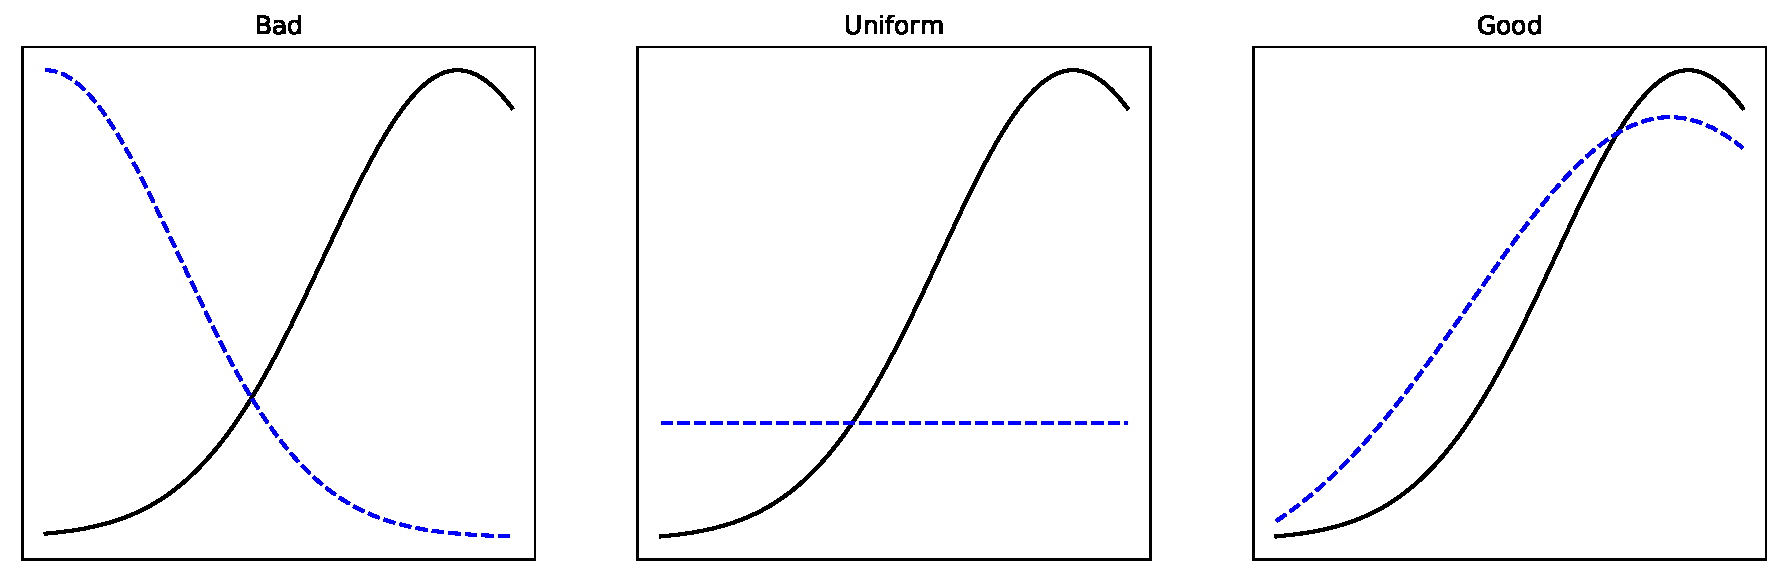
\includegraphics[width=0.8\textwidth]{figures/plots/importancesampling.pdf}
    \caption{The closer $p(x)$ estimates $f(x)$ the more useful the taken samples will be. Less samples $N$ will be needed to effectively calculate a good estimation of $f(x)$.   }
    \label{fig:importancesample}
\end{figure}

\subsection{Multiple Importance Sampling}

When a particular PDF is only suited to sample a certain part of a function, while others may be working for different parts, Multiple Importance Sampling can be used to combine strong densities. Let $n$ be the number of importance sampling strategies, $N_i$ the number of samples for strategy $i$ and $p_i$ the density of the $i$'th strategy. MIS is applied as follows:

\begin{align}
F = \sum_{i=1}^{n}\sum_{j=1}^{N_i}\frac{w_i(x_j)f(x_j)}{N_i \cdot p_i(x_j)}.
\label{eq:mis}
\end{align}

The trivial case is to set constant weights, but this is not optimal as variance essentially adds up. A better approach is for example the Balance Heuristic

\begin{align}
w_i(x_j) = \frac{N_i \cdot p_i(x_j)}{\sum_{k=1}^{n} N_k \cdot p_k(x_j)}.
\label{eq:powerheuristic}
\end{align}

Samples with a higher probability are getting more weight, while samples with small probabilities increase the variance with just $\frac{1}{p_i}$.

\section{Path Tracing}

There are several ways how the rays can actually be traced to solve equation~\ref{eq:req}. Distribution ray tracing \parencite{DBLP:conf/siggraph/CookPC84}, for example, starts one ray and then splits into many rays at each intersection. Other famous variants of ray tracers are Whitted-style ray tracing \parencite{DBLP:journals/cacm/Whitted80}, Bidirectional Path-tracing (BDPT) \parencite{DBLP:conf/rt/LafortuneW96} and Metropolis Light Transport \parencite{DBLP:conf/siggraph/VeachG97}.

We focus our discussions on path tracing even though many concepts can also be adopted to the aforementioned techniques. In path tracing only one indirect light path is continued for each intersection point, although for each pixel many paths are started. This incidentally provides free anti-aliasing when pixel samples are chosen properly. The color of the pixel is calculated by averaging all paths. The segment depth of a path is probabilistically determined by Russian Roulette (RR) to stay unbiased.

\subsection{Next Event Estimation}
\label{sec:NEE}

It is usually too unlikely to hit a light source with a randomly chosen reflection ray, in the case of mass-less point light sources even impossible. The process of deterministically connecting an intersection point with a light source is called Next Event Estimation. Therefor the rendering equation (\ref{eq:req}) has to be split. So far the rendering equation was composed of the emission $L_e$ and reflected radiance $L_r$ as follows:

\begin{align}
L(x, \omega_i) = L_e(x, \omega_i) + L_r(x, \omega_i).
\end{align}

Where $L_r(x, \omega_i)$ is the same as $L_r(y, -\omega_i)$ at the next intersection point $y$. The radiance at $y$ is composed of $L_e$ and $L_r$ as well. Therefor we can split up the reflected radiance into a direct and indirect term.

\begin{align}
L(x, \omega) &= L_e(x, \omega) \\
& \qquad + \int_{\Omega}f_r(\omega_i, x, \omega) L_e(y, -\omega_i)\cos\theta_i \dif\omega_i \\
& \qquad + \int_{\Omega}f_r(\omega_i, x, \omega) L_r(y, -\omega_i)\cos\theta_i \dif\omega_i \\
&= L_e(x,\omega) + L_{\text{direct}}(x, \omega) + L_{\text{indirect}}(x,\omega) \label{eq:reqsplit}
\end{align}

Assuming only one light source, a point light source can now be sampled within the $L_{\text{direct}}$ term as follows. Let $y_l$ be the position of the light, $\omega_{y_l\rightarrow x}$ the vector from $y_l$ to $x$, $V(x,y)$ the visibility between $x$ and $y$ ($1$ when visible, else $0$) and $\Phi_g$ the flux of an isotropic point light, then 

\begin{align}
L_{\text{direct}}(x, \omega) &= \int_{\Omega}f_r(\omega_i, x, \omega) L_e(y, -\omega_i)\cos\theta_i \dif\omega_i \\
&= f_r(\omega_{y_l\rightarrow x}, x, \omega) \frac{\Phi_g}{4\pi||y_l-x||^2} V(x, y_l) \cos\theta_i.
\end{align}

For an area light source we take the integral over its surface $A$

\begin{align}
L_{\text{direct}}(x, \omega) = \int_{A_{LQ}}f_r(\omega_{y \rightarrow x}, x, \omega) L_e(y, \omega_{y \rightarrow x}) G(x,y)V(x,y) \dif A_y.
\end{align}

where $G(x, y)$ is the geometry term

\begin{align}
G(x,y) = \frac{\cos\theta_i\cos\theta_j}{||x-y||^2}.
\end{align}

The integral is numerically estimated with Monte Carlo Integration

\begin{align}
L_{\text{direct}}(x, \omega) \approx \frac{1}{N_s} \sum_{i=1}^{N_s} \frac{f_r(\omega_{y_i \rightarrow x}, x, \omega) L_e(y_i, \omega_{y_i \rightarrow x}) G(x,y_i)V(x,y_i)}{p(y_i)}.
\end{align}

This constitutes a distinct problem (sampling the light source surface) which is necessary for area lights but we explicitly do not address it throughout this work. As such we differentiate between $p_L(k_j)$ which is the probability of choosing the $k_j$-th light source and $p(y_i|k_j)$ which is the probability of choosing point $y_i$ on the $k_j$-th light source. Finally, the direct light is then numerically estimated as

\begin{align}
L_{\text{direct}}(x, \omega) \approx \frac{1}{N_s} \sum_{i=1}^{N_s} \frac{f_r(\omega_{y_i \rightarrow x}, x, \omega) L_e(y_i, \omega_{y_i \rightarrow x}) G(x,y_i)V(x,y_i)}{p_L(k_j)p(y_i|k_j)}.
\end{align}

% The objective of this work is to estimate $p(\omega) \propto L_i(x,\omega_i)$ as good as possible.

\section{Photon Mapping}
\label{sec:PM}
Photon Mapping~\parencite{jensen2001realistic, DBLP:journals/cg/JensenC95} is a quite different approach to solve the rendering equation~\ref{eq:req}. In a first step light sources scatter out photons. These photons are packets of energy, not exactly photons in a physical sense. The flux $\Phi$ of a light source is spread among $N$ photons. Light source and direction is either chosen randomly (uniform) or can be importance sampled with $p_L$ being the probability of choosing the light source $L$ and $p(x,\omega)$ being the probability of choosing the point $x$ and direction $\omega$ on it. The initial power of the photon is then

\begin{align}
\beta = \frac{\Phi_{L,e}(x,\omega)}{p_L \cdot p(x,\omega) \cdot N}.
\end{align}

When the photon hits a surface the BRDF is sampled with Russian Roulette. If the sampled interaction is diffuse or absorbing the photon is saved in the photon map. If it is specular, either reflection or transmission, the photon is continued. The BRDF sampling yields a new direction $\omega_r$ with a probability $p(\omega_r)$. The new power after the reflection then is

\begin{align}
\beta = \frac{\beta \cdot f_r(\omega, y, \omega_r) \cdot \cos\theta}{p(\omega_r)}
\end{align}

The maximum path length can also be limited with RR. With a survival probability $p_s$ a photon is either terminated or continued with power

\begin{align}
\beta = \frac{\beta}{p_s}.
\end{align}

Photons are stored in a balanced k-d tree, so that kNN-searches or radius searches can later be performed efficiently. Either the number of photons $k$ is given and the radius $r$ is set by the outmost photon distance or $r$ is given and $k$ is the number of collected photons. The radiance is then estimated with

\begin{align}
L_r(x, \omega) \approx \frac{1}{r^2\pi} \sum_{p=1}^k f_r(\omega_p, x, \omega) \cdot \beta_p.
\end{align}

The density estimation yields the irradiance $E_i = \frac{Phi}{A}$. The radiance for use in the rendering equation (\ref{eq:req}) then is

\begin{align}
L_i(x, \omega) = \frac{\dif E_i}{\cos\theta_i\dif\omega_i}.
\end{align}

Using the density estimation directly yields very patchy images and is not used in practice. Instead the photon map is either used in a \enquote{Final Gathering} step or in combination with a path tracer, where the photon maps yields the radiance for $L_\text{indirect}$ of the rendering equation in~\ref{eq:reqsplit}. In chapter~\ref{ch:PNEE} we introduce PNEE where the photon map is used as the PDF to importance sample $L_\text{direct}$ instead.

\begin{figure}
    \centering
    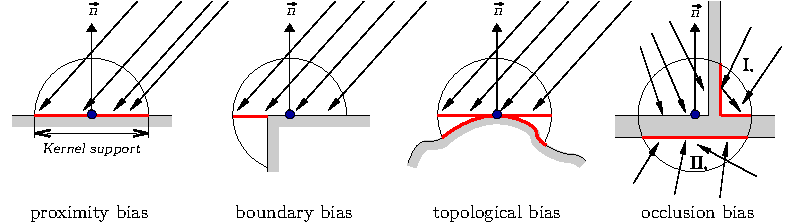
\includegraphics[width=1\textwidth]{figures/biases.pdf}
    \caption{Several biases that occur when collecting photons within the kernel with radius $r$. While the area of collection is assumed to be $r^2\pi$ it can be smaller or larger due to illustrated scenarios.\protect\footnotemark}
    \label{fig:biases}
\end{figure}

\footnotetext{Image taken from~\parencite{lecture}.}
There are several biases, that can occur when photons are collected, illustrated in figure~\ref{fig:biases}. Although the overall technique is consistent, which means it is biased, but it converges against the correct, unbiased solution with an infinite number of photons and thereby infinitesimal search radius. The biases do also play a role in PNEE, for example the occlusion bias can be mitigated with normal culling~\ref{ch:normalculling}. The proximity bias says that the collected photons are not actually (just likely) representative for the current intersection point. This bias is mitigated by weighting the points by distance as we discuss in section~\ref{ch:interpolation}. 

An advanced variant of Photon Mapping is Progressive Photon Mapping (PPM) \parencite{DBLP:journals/tog/HachisukaOJ08} and Stochastic Progressive Photon Mapping (SPPM) \parencite{DBLP:journals/tog/HachisukaJ09}. Instead of storing all photons explicitly, only the radiance estimation and radius is stored is stored per pixel. SPPM extends PPM by replacing the k-d tree a hashed data structure is used. Both techniques might be inspirational for further improvements on PNEE, particularly \textit{photontree} (section~\ref{sec:mixandmatch}).

\section{Data structures}

There exist many data structures with different kind of purposes. In computer graphics data structures are often used to spatially subdivide a three dimensional space. The goal usually is either accelerating construction time, lookup time or memory consumption. The practical efficiency is usually highly dependant on the peculiarities of the scene. A very common problem is high variation in level of detail (LOD), which can be mitigated by adaptive data structures usually at the cost of time and memory in the average case. Imagine a teapot in the middle of a stadium. The teapot is modeled with much detail and the view is focusing on this detail. A rigid spatial data structure might allocate only a fraction of its memory to the teapot, while most of the lookups might be devoted to its detail. We discuss a small selection of relevant data structures in this section. Depending on the application of the data structure e.g. cutting test, traverse or object lookup algorithms are needed. For our case only cell lookups or kNN/radius-searches are relevant. Slight variations in the usage of the data structures commonly exists, we describe our explicit implementation as used for PNEE in chapter~\ref{ch:PNEE}.

\subsection{Grid}
A grid is spatially subdividing the scene in uniformly sized cubes. Therefor the longest dimension of the scene is divided into a given number of cells $k$, the other two dimensions are then filled with the respective cell size. The coordinates of the center are concatenated and hashed. These hashes can now be used in an ordinary hash map to provide $\bigO(1)$ lookups\footnote{Strictly spoken hash map lookups are not guaranteed $\bigO(1)$ but rather depend on the quality of the hashing function.} for the cell. It is convenient when the cell only contains a constant number of elements, at best one. The memory consumption is $\bigO(k^3)$ just for the construction of the cells.

\subsection{Octree}

An Octree starts with a uniform cube that inherits the whole scene. The space is then adaptively subdivided into eight equal sub-cubes when more detail is required in a cell. This is done recursively as long as a threshold isn't reached. A lookup is then made in $\bigO(d)$ where $d$ is the maximal depth of the Octree. Octrees can be effective, but sometimes do not subdivide the space efficiently enough.

\subsection{k-d Tree}

A k-d Tree is a binary tree that recursively subdivides a k-dimensional space with axis-aligned planes. It is a special case of binary space partitioning trees (BSP-tree) where the planes can be chosen arbitrary. At each level an axis is chosen and a plane is fitted so that its sub-space is optimally divided. There are several strategies to choose the \enquote{optimal} split plane. The spatial median divides the space into equal sizes; the construction takes $\bigO(n\log n)$. The object median divides the space so that both branches contain the same number of objects; the construction usually takes $\bigO(n \log^2 n)$ but the tree is balanced therefor. When the k-d tree is supposed to be traversed using a cost function, called Surface Area Heuristic (SAH), is common, where traversing is balanced. Assuming a partition in $k$ spaces a balanced k-d tree uses $\bigO(k \log k)$ memory. The lookup thereof is done in $\bigO(\log k)$. Usually $k$ is proportional but not equal to the number of objects $n$ because a leaf usually contains several objects for efficiency reasons.

\section{Interpolation}

Often a signal is only known at certain data points although we are interested in values that are not given. More precisely, discrete data points of an original function $f(x)$ are given, but we seek to construct a continuous function (interpolant $\widetilde{f}(x)$) or at least certain parts thereof, that matches the original function as much as possible. The resulting function is dependent on assumptions that are inherited in the used interpolation scheme or parametrization. When all given data points are reflected in the function we speak of interpolation, when this is not the case we speak of approximation, although interpolation is used as the hypernym for both. An approximation is usually smoother as extreme points do not have to be matched.

Techniques are usually divided based on whether the data is scattered or structured and whether all given data points (global method) or only adjacent data points (local method) are considered.

\subsection{Scattered data}

One method to handle scattered data is triangulation which subdivides the space into simplices. A Delaunay Triangulation is an assembly of simplices into a convex envelope of all data points without any overlaps. The Delaunay Triangulation is the dual graph to a Voronoi diagram. All points within a Voronoi cell are closer to the cells data point than to any other data point. For a set of data points $S = \{s_i, \dots, s_n \} \in \mathbb{R}^d$ and a distance metric $d(x, y):\mathbb{R}^d \times \mathbb{R}^d \rightarrow \mathbb{R}$ the Voronoi diagram $Vor(S)$ contains a cell $V(s_i)$ for each data points $s_i$ with

\begin{align}
V(s_i) = \{x | d(x,s_i) < d(x,s_j)~\forall j \neq i\}.
\end{align}

Voronoi cells are well illustrated in figure~\ref{fig:voronoi}. There are several algorithms to compute a Delaunay Triangulation in 3D. We evaluated several of them but with a time complexity of usually $\bigO(n^2)$ they were not suitable for our number of data points. 

Another option to interpolate scattered data sets is to use a global method like inverse distance weighting---also called Shepard interpolation. $\widetilde{f}(x)$ with $x \in \mathbb{R}^d$ is calculated from $N$ data points at $x_k \in \mathbb{R}^d$ with its corresponding values $f(x_k)$.

\begin{align}
\widetilde{f}(x) = \sum_{k}^{N}\frac{w_k(x)}{\sum\nolimits_{j}w_j(x)}f(x_k)
\end{align}

with the weight

\begin{align}
w_j(x) = \frac{1}{d(x, x_j)^p}.
\end{align}

We further discuss this interpolation in section~\ref{ch:unstructured}. Another very common approach are Radial Basis Functions (RBF). The weights $\lambda_i$ have to be precomputed with a linear equation system and similar to Shepards weight function the kernel function $\phi$ is an univariate radial basis fuction only dependent on distance $||x-s_i||$. 

\begin{align}
\widetilde{f}(x) = \sum_{i=1}^N \lambda_i \phi(||x - x_i||) + \sum_{m=0}^k c_m p_m (x)
\end{align}

Where a possible kernel is 

\begin{align}
\phi(r) = \mathrm{e}^{-(r/c)^2}
\end{align}

and $p_m$ is an optional polynomial for a $(k+1)$-dimensional vector space in order to enhance interpolation of linear functions.

\subsection{Structured data}
\label{ch:fu:trilinear}

When topological information is already given we speak of structured data. A univariate interpolation can be done with nearest neighbors (0-order), linear (first-order) or smooth (higher-order). For linear interpolation and the point $x$ with $x_i \leq x \leq x_{i+1}$ we define the local coordinate

\begin{align}
u = \frac{x-x_i}{x_{i+1}-x_i}.
\end{align}

The linear interpolant then is

\begin{align}
\widetilde{f}(x) = (1-u)f(x_i) + uf(x_{i+1}).
\end{align}






\begin{figure}
    \centering
    
\includegraphics[width=0.5\textwidth]{figures/img-placeholder.png}
    \caption{The weights are the volume of the opposing rectangle.}
    \label{fig:bilinear}
\end{figure}


\section{Machine Learning}

%\subsection{Light Path Expressions}

%\subsection{Surface Area Heuristic}

%\section{Interpolation}
%\subsection{Scattered data}
%\subsection{Structured data}

%\subsection{Fuzzy k-means}
%\subsection{Agglomerative Hierarchical Clustering}
%\subsection{Expectation Maximaization}
%\subsection{Transductive Support Vector Machine}